% !Mode:: "TeX:UTF-8" 

\BiChapter{基于注意力机制的社交媒体文本立场分析}{Methods of inserting figures}

\BiSection{引言}{Figures inserting standard from graduate school}
当前社交媒体文本立场分析的研究中,研究人员的研究方向主要集中在如何提取社交媒体文本有效的分类特征。忽略了文本立场分析一种重要的出发点是文本基于某个特定的目标,若原文本脱离了特定目标,文本立场分析与情感分析将无差别。基于这个出发点,本章提出了基于条件编码长短期记忆神经网络的模型,通过以条件编码的形式引入文本的目标消息,使立场分析的效果得到显著的提升。本章研究基于条件编码长短期记忆的社交媒体文本立场分析方法,通过以不同形式给模型接入文本立场的目标消息,表明了接入目标信息对文本立场分析有明显提升效果。通过在SemEval2016英文立场分析数据集和NLPCC2016中文立场分析数据集的实验,论证上述结论。

本章的各节结构如下:3.2节介绍条件编码长短期记忆神经网络模型;3.3节介绍基条件编码长短期记忆在文本立场分析;3.4 节为本章实验和结果分析;最后一节为本章小结。

\BiSection{条件编码长短期记忆神经网络模型}{Captions and descriptions of figures}
循环神经网络(Recurrent Neural Networks-RNN)已经在众多自然语言处理任务上取得了巨大成功。不同于传统过得前向反馈神经网络的同层节点无连接层于层之间节点有连接,循环神经网络引入了定向循环,可以处理序列数据。RNN中最大的缺陷是后面时间的节点对于前面节点的感知力下降,当网络深时训练效果下降。LSTM可以解决这一问题,目前LSTM是RNN中使用最广泛最成功的模型。Rocktaschel[???]在2016年在句子之间的文本蕴含识别(Recognizing textual entailment RTE)的研究中提出了条件编码的思想,其论证了在文本含义识别任务上,条件编码比单独编码更能抽取两个句子之间的信息。结合文本立场分析的也有文本和目标需要同时考虑特点,把借鉴条件编码的思想来解决文本立场分析的任务。
\BiSubsection{基于GloVe的词嵌入模型}{}
词的表示是自然语音处理中一个基础且十分重要的任务,大量的研究人员投入到词表示的研究中。早期的有词的表示方式为one hot encoding。每个词独占一个维度,每个词向量有一个维度是1,其他维度为0,词向量的维度是所以单词的的长度。One hot编码的特点是假设所有的单词互相独立,这是一个很强的假设,显然在有些任务中并不合适,如词语相似度方面,dog和cat的相似度应当比dog和not高,但是在one hot编码中他们相似性一样。one-hot编码词表示有一些缺点,如容易受位数灾难的困扰,且不能很好地刻画词与词之间的相似性。词嵌入表示模型能很好的改善one-hot编码的缺点,词的嵌入模型用稠密且固定长度的向量表示每一个词,而且相似的词具有相似的词向量表示。基于这点Mikolov[??]2013提出了Word2Vec模型,解决了词向量训练速度慢,效率低的缺点。其利用了CBOW(Continuous Bag-of-words Model)和Skip-Gram的两种语言模型。其中CBOW的思想是利用词语的上下文词的信息来预测该单词。而Skip-Gram则采取一种和CBOW相反的策略,用中间的词的消息来预测上下文的词。GloVe(Global Vectors for Word Representation)是斯坦福大学发表的一种词嵌入模型,GloVe尝试借鉴NNLM和word2vec的优势来弥补旧方法的劣势,取得了不错的效果。该文发表于word2vec之后,其方法内核比较朴实和简单,官方实验中,GloVe是略胜word2v一筹。

\begin{figure}[htbp]
	\centering
	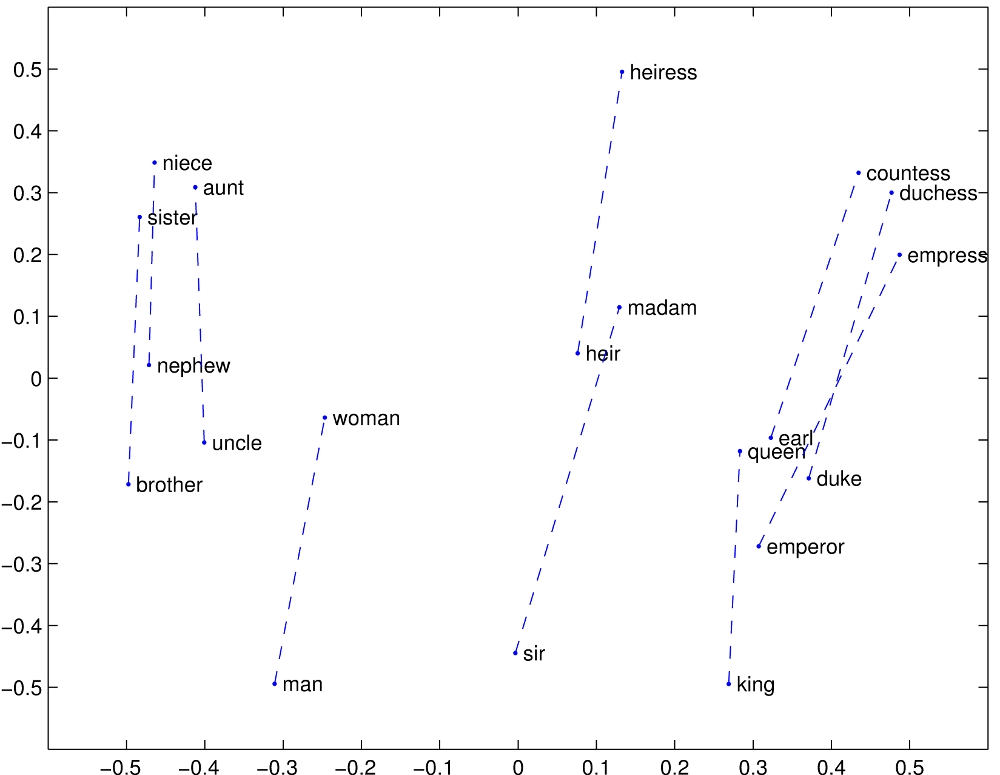
\includegraphics[width = 0.6\textwidth]{glove.jpg}
	\caption[rnn_vanish]{GloVe可视化词向量}
\end{figure}

GloVe结合了基于矩阵分解的词嵌入表示和基于语言模型(例如Word2Vec)的词嵌入表示。基于矩阵分解具有训练快,容易实习的优点,但是生成词向量语义消息十分有限。基于语言模型的词嵌入表示则具有更多语言学层次的支持,在更多自然语言处理任务上表现更好,但是模型关注的上下文特征较少,忽略了全局的信息。GloVe发明的初衷,就是想结合两者的长处,建立一个充分利用统计量的更好训练的适用程度更广的词嵌入模型。具体模型建立公式如下

$$ F(w_i,w_j,w^c_k) = \cfrac{P_{ij}}{P_{jk}} $$
其中,取$word_i$的出现次数为$X_i$, 定义$P_{ij}=P(j|i)=\cfrac{X_{ij}}{X_{i}}$表示在$X_i$的上下文下$word_i$的出现几率, $F$则是某一种能够实现我们需求的变换。$w_i,w_j$是实数空间下的$word_i,,word_j$的词向量,$w^c_k$也是实数空间下的$word_k$的上下文词向量,其作用类似word2vec中的上下文向量。为了精简计算引入词向量的线性加减和点乘计算
$$ F((w_i-w_j)^Tw^c_k) = \cfrac{F(w^T_iw^c_k)}{{F(w^T_jw^c_k)}} $$
GloVe每个词涉及到两个词向量,一个词语本身的向量$w_i$,一个词的context向量$w^c_i$。最初这样设计,将词向量和上下文的向量分开,不用一套,是为了在更新参数的时候能够简单地套用SGD。实验证明两个向量加起来最后起到的效果最好。后面英文的词向量用的是GloVe模型在大量的Twitter文本上训练的100维度的词向量,中文微博词向量是200维度的词向量。

\BiSubsection{长短期记忆神经网络模型}{Layouts of illustrations}
由于文本序列的通常具有较长的长度,导致神经网络的层数较多,而传统的递归神经网络解决序列问题经常会出现梯度消失的问题(vanishing gradient problem)与梯度爆炸问题(gradient exploding problem)。梯度消失问题和梯度爆炸问题一般随着网络层数的增加会变得越来越明显。出现的原因在于对神经网络参数进行链式求导的过程中,输出对于前面递归神经参数的倒数随着累乘激活函数的导数而接近于0,以下图的反向传播为例(假设每一层只有一个神经元且对于每一层$y_i=\sigma(z_i)=\sigma(w_ix_i+b_i)$,其中$\sigma$为sigmoid函数)

\begin{figure}[htbp]
	\centering
	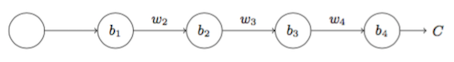
\includegraphics[width = 0.7\textwidth]{rnn_gradient_vanish.png}
	\caption[rnn_vanish]{RNN梯度消失}
\end{figure}

可以推导出

\begin{equation}\label{nodelimiter}
\frac{\partial C}{\partial b_1} = \frac{\partial C}{\partial y_4}\frac{\partial y_4}{\partial z_4}\frac{\partial z_4}{\partial x_4}\frac{\partial x_4}{\partial z_3}\frac{\partial z_3}{\partial x_3}\frac{\partial x_3}{\partial z_2}\frac{\partial z_2}{\partial x_2}\frac{\partial x_2}{\partial z_1}\frac{\partial z_1}{\partial b_1}
\end{equation}
\begin{equation}\label{delimiter}
=\frac{\partial C}{\partial y_4}\ \sigma ^\prime(z_4)w_4\sigma ^\prime(z_3)w_3\sigma ^\prime(z_2)w_2\sigma ^\prime(z_1)
\end{equation}

一般的非线性激活函数的导数都小于1(例如sigmoid的导数最大值为$\frac{1}{4}$),因此对于上面的链式求导,层数越多,求导结果$\frac{\partial C}{\partial b_1}$越小,因而导致梯度消失的情况出现。
长短期记忆(Long Short-Term Memory, LSTM)是一种缓解上述问题的间递归神经网络的变种,Hochreiter在1997年首次提出了LSTM结构,2000年Gers等人改进LSTM模型。

\begin{figure}[htbp]
	\centering
	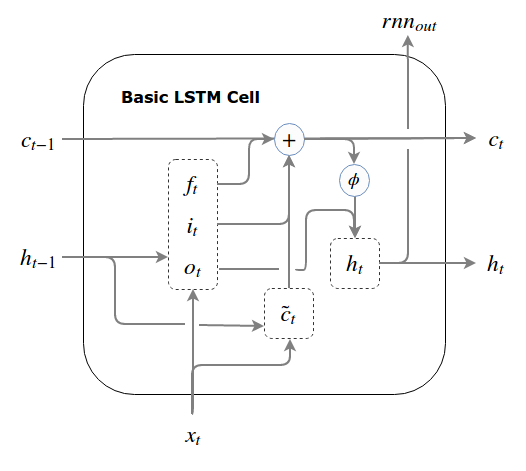
\includegraphics[width = 0.6\textwidth]{lstm_unit.png}
	\caption[rnn_vanish]{LSTM单元结构}
\end{figure}

LSTM模型提出了记忆存储格(memory cell)的结构,内部包含了遗忘门(forget gate)、输入门(input gate) 和输出门(output gata) 。各种门的作用在于调节记忆体在外部输入的情况下应该采取怎么的存储测量,具体门状态和记忆体内部参数的更新公式如下。

\begin{equation}\label{lstm_f}i_t=\sigma_g(W^ix_t+U_ih_{t-1}+b^i)\end{equation}
\begin{equation}\label{lstm_f}f_t=\sigma_g(W^fx_t+U_fh_{t-1}+b^f)\end{equation}
\begin{equation}\label{lstm_f}o_t=\sigma_g(W^ox_t+U_oh_{t-1}+b^o)\end{equation}
\begin{equation}\label{lstm_f}c_t=f_t \odot c_{t-1}+i_t\odot \sigma_c(W_cx_t+U_ch_{t-1}+b_c)\end{equation}
\begin{equation}\label{lstm_f}h_t=o_t \odot \sigma_h(c_t)\end{equation}

其中$\sigma_g$为sigmoid的激活函数,$\sigma_c, \sigma_h$为thah的激活函数,$x_t$为输入向量,$h_t$为输出向量, $c_t$为记忆向量,$W,U,b$是矩阵参数和向量参数。各个门的值是保持在0-1之间的向量。其中遗忘门向量$f_t$表示上一时刻的记忆体信息需要遗忘多少, 输入门向量$i_t$表示有多少当前时刻输入信息需要加入到记忆体中,输出门向量$o_t$表示记忆体输出多少信息。

前已经证明,LSTM是解决长序依赖问题的有效技术,并且这种技术的普适性非常高,导致带来的可能性变化非常多。各研究者根据LSTM纷纷提出了自己的变量版本,这就让LSTM可以处理千变万化的垂直问题

\BiSubsection{条件编码长短期记忆神经网络模型}{}
Rocktaschel[]等在句子之间的文本蕴含识别的研究中提出了条件编码长短期记忆神经网络模型,文本蕴含定义为一对文本之间的有向推理关系,其中蕴含前件记作T(Text),蕴含后件记作H(Hypothesis)。如果人们依据自己的常识认为H的语义能够由T的语义推理得出的话,那么称T蕴含H,记作T → H, 作者提出的模型的结构是首先有一个LSTM模型编码Text消息,另一个不同参数的LSTM模型编码Hypothesis。作者不是简单把两个特征向量拼接在一起,而是做了如下转换。把第一个编码Text信息的LSTM模型的记忆状态(Cell)保留下来,作为第二个编码Hypothesis的LSTM模型记忆状态(Cell)的初始值,此模型建立的了Text消息作为条件下的对Hypothesis的编码表示。

\begin{figure}[htbp]
	\centering
	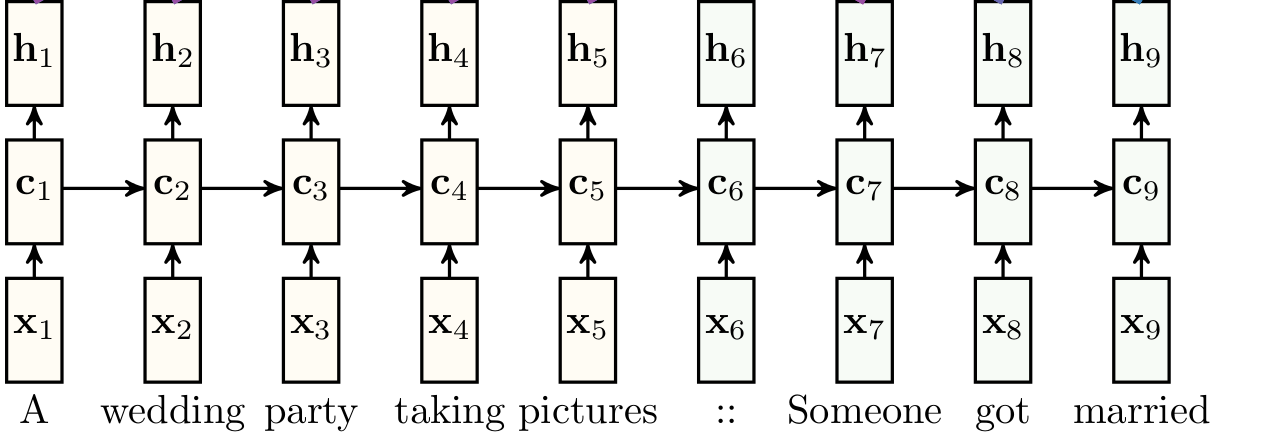
\includegraphics[width = 0.8\textwidth]{conditional_encoding.png}
	\caption[rnn_vanish]{条件编码长短期记忆}
\end{figure}

如上图图表示所示“A wedding party taking pictures”作为我们的Text文本,“Someone got married”作为我们的Hypothesis,其中$c_5$作为前一个LSTM的记忆体状态被当做编码Hypothesis的初始记忆状态。两个LSTM具体的状态转移公式如下:
\begin{equation}\label{lstm_f}[h_1~c_1] = LSTM^{Text}(x_1,h_0,c_0)\end{equation}
$$...$$
\begin{equation}\label{lstm_f}[h_T~c_T] = LSTM^{Text}(x_1,h_{T-1},c_{T-1})\end{equation}
\begin{equation}\label{lstm_f}[h_{T+1}~c_{T+1}] = LSTM^{Hypothesis}(x_1,h_0,c_T)\end{equation}
$$...$$
\begin{equation}\label{lstm_f}[h_{N}~c_{N}] = LSTM^{Hypothesis}(x_1,h_{N-1},c_{N-1})\end{equation}
\begin{equation}\label{lstm_f}c=tanh(Wh_N)\end{equation}
其中$(x_1...x_T)$为Text的序列消息,$(x_{T+1}...x_N)$为Hypothesis的序列信息。$h_0,c_0$为LSTM的初始化向量。

实验证明在文本蕴含任务上,条件LSTM模型比单独编码高3.3\%(从77.6\%提升到80.9\%)的性能。这种条件编码能使Text的信息更好的流向对Hypothesis编码的LSTM模型,有了第一个LSTM模型传来的记忆状态,第二个LSTM模型能更好的编码Hypothesis的消息。

\BiSection{基于条件编码长短期记忆的文本立场分析}{}

通过Rocktaschel在文本蕴含的任务的实验可知,在处理两个文本序列的编码任务上,条件编码长短期记忆神经网络比单独独立编码两个文本序列有更好的建模能力。在文本立场分析的任务上,有文本的信息和目标主题两个文本序列信息,我们可以借鉴条件编码长短期记忆神经网络在文本蕴含建模的方式,把文本信息和目标主题信息更好结合起来。在实验部分设计了多种文本序列信息的结合方式,通过实验证明了以目标主题文本作为条件编码文本信息的模型对文本立场分析有更好的效果。

本文后期实验将在NLPCC2016中文微博立场分析数据集和SemEval2016英文Twitter立场分析数据集,为较清晰阐述条件编码长短期记忆模型,以下简短的介绍下两个数据集的样例,具体的有关数据集的信息将会在下面实验部分做详细介绍。

例1:目标主题文本:"深圳禁摩限电" 微博文本:"支持深圳交警。电单车继续治理" 立场分析类标:“Favor”(持支持立场)

目标的文本主题有关“深圳禁摩限电”的主题的,而从微博文本“支持深圳交警。电单车继续治理”中,我们可以知道微博的作者首先是赞同了深圳交警的行为,然后叙述了电单车需要得到继续的整治,从两个方法肯定了"深圳禁摩限电"这个主题目标的,因此给出的类标是“Favor”也就是持支持目标主题的立场。

例1:目标主题文本:"Hillary Clinton" Twitter文本:"Hopefully Hillary Clinton gets cancer and dies before she gets the opportunity to embarrass our country any further“,立场分析类标“Against”(持反对立场)

译文:"真希望希拉里克林顿得癌症然后死去,这样她就不再会有机会再让我们国家蒙羞了。"

目标的文本主题有关“希拉里克林顿”的主题的,这个Twitter文本是有关2016年美国大选,显然Twitter作者一直咒骂希拉里克林顿,希望她得癌症,不让她侮辱国家,可以看出作者有强烈反对主题目标“希拉里克林顿”,因此给出的类标是“Against”,也就是持反对目标主题的立场。

从上述的两个简单的样例可知,立本立场是有两个输入的,一个是立场主题例如“深圳禁摩限电”和“Hillary Clinton”。另外一个是立场下的文本“支持深圳交警。电单车继续治理”和”Hopefully Hillary Clinton gets cancer and dies before she gets the opportunity to embarrass our country any further“。在这通过中文微博阐述条件编码长短期记忆模型的建立。首先经过一些数据预处理和分词把主题目标”深圳禁摩限电“和”支持深圳交警。电单车继续治理”转变成”深圳 禁摩 限电“和”支持 深圳 交警 电单车 继续 治理“。

在文本立场分析的任务, 一般目标主题包含的信息较少,而文本包含了大部分的信息。例如上面两个例子所举例的,目标主题文本分别为”Hillary Clinton“和”深圳禁摩限电“,而Twitter和微博文本包含的消息较多,结合立场分析文本的特点,改善了原有的条件编码长短期记忆的网络结构,后续实验论证在多种条件编码长短期记忆的改进方案中,下面所示的网络结构具有更好的实验效果,后续在实验分析其可能的原因。

\begin{figure}[htbp]
	\centering
	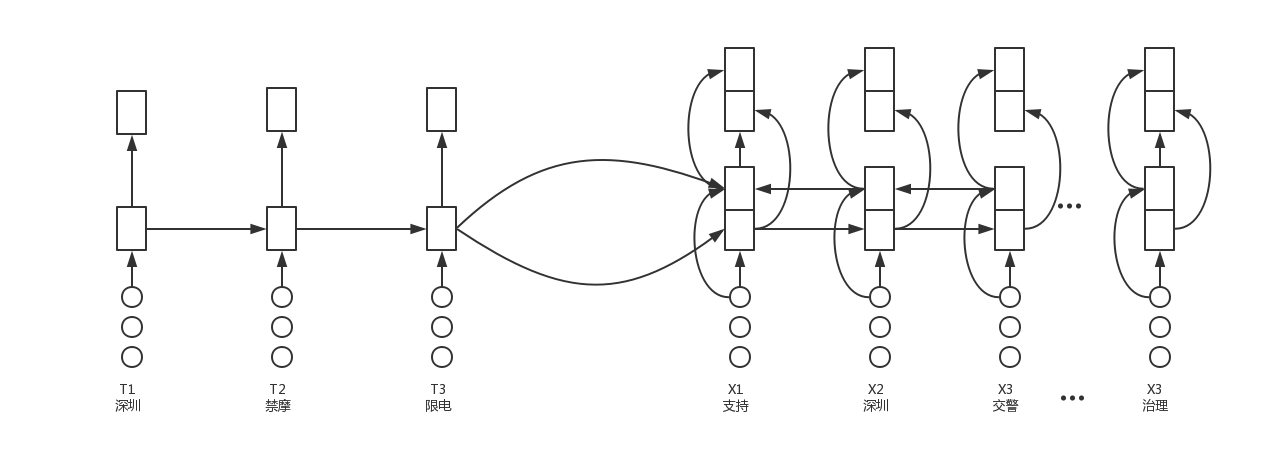
\includegraphics[width = 1.0\textwidth]{conditional_encode_lstm.png}
	\caption[rnn_vanish]{条件编码长短期记忆}
\end{figure}

模型的具体公式如下

\begin{equation}\label{lstm_f}[h_1~c_1] = LSTM^{target}(t_1,h_0,c_0)\end{equation}
$$...$$
\begin{equation}\label{lstm_f}[h_M~c_M] = LSTM^{target}(t_1,h_{M-1},c_{M-1})\end{equation}

\begin{equation}\label{lstm_f}[h^{forward}_{1}~c^{forward}_{1}] = LSTM^{forward}(x_1,h_0,c_T)\end{equation}
$$...$$
\begin{equation}\label{lstm_f}[h^{forward}_{N}~c^{forward}_{N}] = LSTM^{forward}(x_n,h^{forward}_{N-1},c^{forward}_{N-1})\end{equation}

\begin{equation}\label{lstm_f}[h^{backward}_{N}~c^{backward}_{N}] = LSTM^{backward}(x_n,h_0,c_T)\end{equation}
$$...$$
\begin{equation}\label{lstm_f}[h^{backward}_{1}~c^{backward}_{1}] = LSTM^{backward}(x_1,h^{backward}_{2},c^{backward}_{2})\end{equation}

\begin{equation}\label{lstm_f}c_i=Softmax(W[h^{forward}_n~h^{backward}_1])\end{equation}

其中$M$为主题目标的文本长度,$N$为微博()Twiiter的文本长度。$LSTM$单向编码主题目标,$LSTM^{forward}$为前向编码文本信息,$LSTM^{backward}$为后向编码文本信息,$h_0$为LSTM的初始化向量,$C_T$为$LSTM$主题目标编码的最后一个Cell状态,$h^{backward}_{1},h^{forward}_{N}$分别为前向和后向编码的最后一个隐藏状态。

本节以“深圳禁摩限电”为话题目标,微博文本“支持深圳交警。电单车继续治理”为例,按本节模型的 4 个层次,描述基于条件编码长短期记忆的立场分析的过程。

(1)输入层

先将话题目标和微博文本经过预处理操作,然后通过分词工具把话题目标和微博文本进行划分,对于同一个话题目标,微博文本分词后句子长度有可能不一致,为了方便后续神经网络框架中的批量的并行计算,通过统计选择30为固定长度,长度超过固定长度进行截断操作,不够的进行补齐词表中规定<PAD>关键词。如例微博文本最后转换成”支持 深圳 交警。电单车 继续 治理 <PAD> ... <PAD>“

(2)词向量嵌入层

词向量的嵌入层,此层的功能是对输入的每一次词检索其词向量(lookup操作),后续实验词向量的预训练由GloVe模型在大量无监督语料上训练可得,预训练的词向量维度为100,且把词向量设置为可训练,随神经网络模型的训练动态调整权重。

(3)主题目标编码层

通过一个单向的长短期记忆(LSTM)模型模型编码主题目标,把分词后的主题目标“深圳 禁摩 限电”通过lookup操作取出相应的词向量,经过一个隐藏层为64的单向LSTM模型,且保留最后的记忆体的状态,如上图所示,保留XXX的单元的信息,给下一层文本编码做输入。

(4)文本编码层

由于文本包含大部分信息,所以采用了双向的LSTM模型而不是Rocktaschel提出的单向的LSTM模型编码文本信息。如上图所示,文本编码的双向LSTM模型的初始Cell状态是由上一层的目标主题编码的最后的Cell状态填充,表示主题目标的消息流入到当前的双向LSTM模型中参与对文本的编码操作。每一个方向LSTM的最后的隐状态h作为对整个文本的最终编码表示。

(5)全连接层


全连接层接受来自文本编码层每个方向最后的隐状态,拼接两个隐状态信息作为最后的特征向量。全连接层的输出个数为3,表示每个立场的预测概率。通过softmax激活函数归一化三个立场的概率,在预测阶段我们选取概率最大的立场当做预测的类标。

\BiSection{实验结果及分析}{hello}

本节主要介绍条件编码长短期记忆神经网络模在2016NLPCC微博中文语料库和2016SemEval英文Twitter数据集中的实验结果及分析。并从实验的角度论证条件编码长短期记忆在立场分析问题上的有效性。本节包含两部分: 3.4.1 小节介绍中英文两个数据集中训练和测试文本的分布 、实验评价方式以及对比方法;3.4.2 小结介绍模型训练阶段的性能调优,以及本章实验与其他方法的比较。

\BiSubsection{实验数据与评价指标}{}

(1)数据集简介

为验证条件编码长短期记忆神经网络在立场分析任务上算法的性能表现,本节采用2016 NLPCC中文微博语料和2016 SemEval英文的Twitter语料两个数据集验证算法的效果。以下分别介绍两数据集的分布。

中文数据集来自NLPCC2016 立场分析测评任务[55] ,数据集的5个话题目标分别为 iPhone SE、春节放鞭炮、俄罗斯在叙利亚的反恐行动、开放二胎政策和深圳禁摩限电。所有语料都来自于新浪微博,每个微博文本的立场属于“支持”、“反对”和“其他”三者之一。NLPCC 2016中文微博数据集的训练集、测试集按照75\%与25\%的比例划分,如表~\ref{chinesedata}~所示详细介绍每个话题目标下数据的分布。
\begin{table}[htbp]
	\caption[table123]{训练集、测试集话题数量及立场分布比例(中文数据集)}
	\label{chinesedata}
	\vspace{0.5em}\centering\wuhao
	\begin{tabular}{cccccccccc}
		\toprule[1.5pt]
		\multirow{2}{*}{预置话题分类}& \multicolumn{4}{c}{训练集数量和立场比例(\%)} 
		& \multicolumn{4}{c}{测试集数量和立场比例(\%)}  &\multirow{2}{*}{文本数量}\\
		\cline{2-9}
		\quad&数量& 支持&反对&其他&数量& 支持&反对&其他 \\
		\midrule[1pt]
		iPhone SE&600&40.8&34.8&24.3&200&37.5&52.0&10.5&800\\
		春节放鞭炮&600&41.7&41.7&16.7&200&44.0&47.0&9.0&800\\
		俄在叙反恐行动&600&41.7&41.7&16.7&200&47.0&43.0&10.0&800\\
		开放二胎政策&600&43.3&33.3&23.3&200&49.5&47.5&3.0&800\\
		深圳禁摩限电&600&26.7&50.0&23.3&200&31.5&55.0&13.5&800\\
		总计&3000&38.8&40.3&20.9&1000&41.9&48.9&9.2&4000\\
		\bottomrule[1.5pt]
	\end{tabular}
\end{table}

英文数据集来自SemEval2016 Task6 stance detection[55] ,数据集的5个话题目标分别为 Atheism(无神论)、Climate Change is a Real Concern(气候变化真实性)、Feminist Movement(女权运动)、 Hillary Clinton (希拉里克林顿)和
Legalization of Abortion(堕胎合法化)。所有语料都来自于英文Twitter文本,每个Twitter文本的立场属于“支持”、“反对”和“其他”三者之一。不同于上述中文语料的分布,每个话题目标英文Twitter语料的数量参差不齐,但总体上训练集和测试集按70\%与30\%的比例划分,如表~\ref{englishdata}~所示详细介绍每个话题目标下数据的分布。


\begin{table}[htbp]
	\caption[table123]{训练集、测试集话题数量及立场分布比例(英文数据集)}
	\label{englishdata}
	\vspace{0.5em}\centering\wuhao
	\begin{tabular}{cccccccccc}
		\toprule[1.5pt]
		\multirow{2}{*}{预置话题分类}& \multicolumn{4}{c}{训练集数量和立场比例(\%)} 
		& \multicolumn{4}{c}{测试集数量和立场比例(\%)}  &\multirow{2}{*}{文本数量}\\
		\cline{2-9}
		\quad&数量& 支持&反对&其他&数量& 支持&反对&其他 \\
		\midrule[1pt]
		Atheism&513&17.9&59.3&22.8&220&14.5&72.7&12.7&733\\
		Climate Change&395&53.7&3.8&42.5&169&72.8&6.5&20.7&564\\
		Feminist Movement&664&31.6&49.4&19.0&285&20.4&64.2&15.4&949\\
		Hillary Cliton&689&17.1&57.0&25.8&295&15.3&58.3&26.4&984\\
		Legal of Abortion&653&18.5&54.4&27.1&280&16.4&67.5&16.1&933\\
		总计&2914&25.8&47.9&26.3&1249&24.3&57.3&18.4&4163\\
		\bottomrule[1.5pt]
	\end{tabular}
\end{table}

为了和已有方法进行性能比较,本文在两数据集上都按照分别测评的比例划分出训练集和测试集。其中训练集负责模型的训练和调优, 测试集则进行最后模型的性能的评估。中英文数据集均包含5个不同的话题目标, 每个话题目标包含若干的话题文本,由于每个主题目标关注的内容不同且具有各自独特的语言特点。为了使模型更好的拟合每一种话题的特性,本文首先按照中英文不同语料集合划分成两个大任务,然后根据每个语料库在细分成5个不同子任务,分别建立不同的条件编码长短期记忆模型。各子模型预测结束后, 统计各个子任务上的性能并汇总预测结果进行最后统一指标的计算。

(2)评价指标

中英文数据集上的社交媒体文本的立场结果有“支持”,“反对”,“其他”,可以把任务当成一个三分类任务,但是由于三个类在不同的数据集下的不同主题目标的分布有可能很不平均,如果只单独用正确率(Accuracy)作为评测指标则缺失了评价指标的客观性。本文c采取了两个评测任务都使用的”支持“和”反对“的F1指标的微平均(micro-average)作为最后模型的评测指标,但是为了更清晰的评价每个主题目标的性能,每个目标主题也会单独计算微平均评测指标。为了清晰地解释指标的含义,列举以下公式说明

首先定义准确率(Precision, P)、召回率(Recall, R),如公式~\ref{precision}~和公式~\ref{recall}~所示。
\begin{equation}\label{precision}P=\frac{TP}{TP+FP}\end{equation}
\begin{equation}\label{recall}F=\frac{TP}{TP+FN}\end{equation}

TP:正样例预测为正样例的个数

FP:负样例预测为正样例的个数

FN:正样例预测为负样例的个数。

精确率计算的是所有"正确被检索的样例(TP)"占所有"实际被检索到的(TP+FP)样例的比例。召回率计算的是所有"正确被检索的运力(TP)"占所有"应该检索到的样例(TP+FN)"的比例。如果要同时考虑精确率和召回率,则需要采样两者的调和平均值,也称为F1值,其定义如公式~\ref{f1score}~所示
\begin{equation}\label{f1score}F1=\frac{2PR}{P+R}=\frac{2TP}{2TP+FP+FN}\end{equation}

有关”支持“立场F1值的计算,“支持”类标作为正样本,“反对”后“其他”作为负样本。因此其计算公式如下所示

\begin{equation}\label{f1favor}F1_{favor}=\frac{2P_{favor}R_{favor}}{P_{favor}+R_{favor}}\end{equation}

同样的”反对“立场F1值的计算,“反对”类标作为正样本,“支持”后“其他”作为负样本。因此其计算公式如下所示

\begin{equation}\label{f1against}F1_{against}=\frac{2P_{against}R_{against}}{P_{against}+R_{against}}\end{equation}

立场分析总的平均指标F1的微平均(Micro-average)的计算公式如下
\begin{equation}\label{f1average}F1_{average}=\frac{F1_{favor}+F1_{against}}{2}\end{equation}

为论证在立场分析中,合理利用主题目标的信息能提高立场分析的性能,设计了以下模型。

用LSTM直接编码文本Text信息,不引入主题目标信息,以下简称\textbf{Text-Only}。

用两个不同LSTM模型分别编码主题目标Target和文本Text信息,两个LSTM独立编码各自的信息,最后拼接两者的编码向量作为最后参与分类的特征向量,以下简称\textbf{Text-Target}。

用两个不同LSTM模型分别编码主题目标Target和文本Text信息,对主题目标Target最后LSTM模型的记忆单元(Cell)状态做为对文本编码LSTM模型的初始状态,构成以主题目标Target为条件的Text文本编码,取Text编码LSTM的最后一个隐状态作为最后的特征向量,以下简称\textbf{Text-on-Target}。

针对立场分析数据的特点,主题目标所包含的信息相对有限,而文本包含绝大部分信息的特点。改进了条件编码的模型,与(3)相同用单向的LSTM编码主题目标信息,为了充分提取文本的信息,采用双向LSTM模型来提取文本的信息,类似于(3)的做法,编码文本的双向LSTM模型的记忆单元来自于对主题目标编码的LSTM的最后记忆单元状态,以下简称\textbf{BiText-on-Target}。

首先为了初步验证主题目标的信息对立场分析是否具有提升作用,通过对比Text-Only和Text-Target模型的性能可以初步得出主题目标的信息对立场分析是否有促进作用,然后为了进一步说明条件编码LSTM模型是否能跟好的利用主题目标的消息参与对文本的编码,设计了Text-Target模型和Text-on-Target模型的对比实验。最后为了对比我们改进过了的条件编码BiText-on-Target模型是否能更好编码文本信息,设计了Text-on-Target模型和BiText-on-Target模型的对比实验。

\BiSubsection{实验数据预处理与模型参数设计}{}

本文实验的社交媒体立场分析数据都来自于新浪微博或者Twitter,此类网络语言文本具有文本形式极度不规范,口语化严重。Twitter与微博是由网络用户即兴创作的短文本,用户在用词、语法等方面随意性较大,文本形式与新闻、维基百科等语料具有很大的差异。由于Twitter和微博一般有对单条文本长度做出文本长度的限制,因此这些网络文本中常含有缩写、俗语、流行词汇等元素,同样也存在语法成分缺失的问题。除此之外,文本中大量存在的网页链接、“@某用户”和“\#某话题”等功能标记。

由于社交媒体文本根据上述特点,分别对中英文语句进行预处理操作。删除语料中其中的大量URL信息,由于“\#某话题”等话题标签对立场分析有很重要的影响,因此把话题标签消息保留了下来,对于英文所有词语全转换成小写拼写,分词工具采用了CMU专门为Twitter开发的Twitter NLP tool里面的分词模型[XXX], 中文的分词工具采用较为稳定的结巴分词工具。对于网络社交文本分词后可转换成一些词语的序列信息,对于在训练集中出现次数小于2词的词语归为低频词,为了减少模型的参数,加大模型的泛化能力,把所以的低频词转换成一个统一的词汇用“UNKNOW”标识。同时为了兼容现在主流的基于批量更新的深度学习框架,对文本的长度进行固定操作。英文的文本固定为30个词的长度,中文微博文本固定为50的词长度。

英文语料的词向量训练通过GloVe算法在20亿Twitter文本语料训练而成,其中包含了120万个词,词向量维度为200。中文微博语料是通过Word2Vec算法在大量微博语料中训练所得,其中包含了17万个词,词向量的维度也为200。

本文建立了针对5个不同话题目标的子模型, 使用相同的条件编码长短期记忆模型参数。取出训练集合的10\%作为验证集参与模型的选择。通过实验发现,当对主题目标和文本编码LSTM模型的隐藏层单元设置为64,embedding层的dropout的概率设置为0.2,当对主题目标和文本编码LSTM模型内部记忆的dropout概率设置为0.3,每次以32个样本作为mini-batch参加参数更新,选取0.001的学习率的Adam优化方法。

\begin{table}[htbp]
	\caption[param]{基于条件双向编码长短期记忆的立场分析实验超参数集}
	\label{param}
	\vspace{0.5em}\centering\wuhao
	\begin{tabular}{ccc}
		\toprule[1.5pt]
		序号& 超参数名称 &数值\\
		\midrule[1pt]
		1 &LSTM隐藏层单元& 64\\
		2 &Embedding层dropout& 0.2\\
		3 &LSTM内部drought& 0.3\\
		4 &批处理大小& 32\\
		5 &L2 正则化参数 &1e-6\\
		6 &全量迭代次数& 50\\
		7 &梯度优化方法& Adam\\
		8 &学习率& 0.001\\
		\bottomrule[1.5pt]
	\end{tabular}
\end{table}

\BiSubsection{模型对比实验结果及分析}{}
通过在
\begin{table}[htbp]
	\caption[table123]{基于子话题分别训练的条件双向编码长短期记忆模型试验性能(SemEval数据集)}
	\label{chinesedata}
	\vspace{0.5em}\centering\wuhao
	\begin{tabular}{cccccccc}
		\toprule[1.5pt]
		预置话题分类& $P_{favor}$&$R_{favor}$&$F_{favor}$&$P_{against}$&$R_{against}$&$F_{against}$&$F_{average}$ \\
		\midrule[1pt]
		iPhone SE&600&40.8&34.8&24.3&200&37.5&52.0\\
		春节放鞭炮&600&41.7&41.7&16.7&200&44.0&47.0\\
		俄在叙反恐行动&600&41.7&41.7&16.7&200&47.0&43.0\\
		开放二胎政策&600&43.3&33.3&23.3&200&49.5&47.5\\
		深圳禁摩限电&600&26.7&50.0&23.3&200&31.5&55.0\\
		总计&3000&38.8&40.3&20.9&1000&41.9&48.9\\
		\bottomrule[1.5pt]
	\end{tabular}
\end{table}

\begin{table}[htbp]
	\caption[table123]{基于子话题分别训练的条件双向编码长短期记忆模型试验性能(NLPCC数据集)}
	\label{chinesedata}
	\vspace{0.5em}\centering\wuhao
	\begin{tabular}{cccccccc}
		\toprule[1.5pt]
		预置话题分类& $P_{favor}$&$R_{favor}$&$F_{favor}$&$P_{against}$&$R_{against}$&$F_{against}$&$F_{average}$ \\
		\midrule[1pt]
		iPhone SE&600&40.8&34.8&24.3&200&37.5&52.0\\
		春节放鞭炮&600&41.7&41.7&16.7&200&44.0&47.0\\
		俄在叙反恐行动&600&41.7&41.7&16.7&200&47.0&43.0\\
		开放二胎政策&600&43.3&33.3&23.3&200&49.5&47.5\\
		深圳禁摩限电&600&26.7&50.0&23.3&200&31.5&55.0\\
		总计&3000&38.8&40.3&20.9&1000&41.9&48.9\\
		\bottomrule[1.5pt]
	\end{tabular}
\end{table}

